\section{Auswertung}
\label{sec:Auswertung}

Die Graphen werden sowohl mit Matplotlib \cite{matplotlib} als auch NumPy \cite{numpy} erstellt. Die Fehlerrechnung wird mithilfe von Uncertainties \cite{uncertainties} durchgeführt.

\subsection{Bestimmung der Reichweite von Alpha-Strahlung Messung 1}

Bei der ersten Messung ist die Probe $\SI{2.7}{\centi\metre}$ vom Detektor entfernt.
In Abbildung \ref{fig:1N} ist mit den Werten aus Tabelle \ref{tab:1} die Impulsrate $N_1$ der ersten Messung gegen die effektive Laufzeit $x_.{eff1}$ aufgetragen, welche nach Formel \eqref{eq:x} bestimmt wird.
Mittels einer linearen Ausgleichsrechnung der Form $N(x_.{eff})=a x_.{eff} +b$ im Bereich von $x_.{eff1} = \SI{17.3}{\milli\metre}$ bis $x_.{eff1} = \SI{22.7}{\milli\metre}$ ergibt sich die mittlere Reichweite $R_m$:
\begin{align*}
a	&= \SI{-114(4)}{\becquerel\per\milli\per\metre}\text{,}\\
b	&= \SI{2.68(9)e3}{\becquerel}\text{,}\\
R_m	&= \frac{N_{1/2}-b}{a} = \SI{19(1)}{\milli\metre}\text{.}
\end{align*}
Dabei ist $N_{1/2} = \SI{530}{\becquerel}$ und der Fehler $\sigma_{R_m}$ von $R_m$ berechnet sich mit der Gaußschen Fehlerfortpflanzung nach:
\begin{equation*}
\sigma_{R_m} = \sqrt{\left(\frac{N_{1/2}-b}{a^2}\sigma_a\right)^2+\left(\frac{1}{a}\sigma_b\right)^2}\text{.}
\end{equation*} 
Mithilfe von $R_m$ lässt sich die Energie $E_\alpha$ der Alphateilchen mit Formel \eqref{eq:Rm} bestimmen zu:
\begin{equation*}
E_\alpha = \SI{3.3(1)}{\mega e\volt}\text{.}
\end{equation*} 
Der Fehler $\sigma_{E_\alpha}$ bestimmt sich dabei nach:
\begin{equation*}
\sigma_{E_\alpha} = \frac{2}{9,3}\left(\frac{R_m}{3,1}\right)^{-\frac{1}{3}}\sigma_{R_m}\text{.}
\end{equation*} 
In Abbildung \ref{fig:1E} ist mit den Werten aus Tabelle \ref{tab:1} die Energie $E_1$ der ersten Messung gegen die effektive Laufzeit $x_.{eff1}$ aufgetragen.
Mittels einer linearen Ausgleichsrechnung der Form $E(x_.{eff})=m_1 x_.{eff} +n_1$ ergibt sich für den Energieverlust $\frac{.dE_1}{.dx}$:
\begin{align*}
\frac{.dE_1}{.dx}	&= m_1 = \SI{-91(3)}{\mega e\volt\per\metre}\text{,}\\
n_1	&= \SI{3.74(4)e6}{\becquerel}\text{.}
\end{align*}

\begin{table}
	\centering
	\caption{Der Druck $p$ und die Impulsrate $N_1$, sowie die effektiven Längen $x_.{eff1}$ und die bestimmten Energien $E_1$ bei der ersten Messreihe mit einem Abstand zur Probe von $\SI{2.7}{\centi\metre}$.}
	\label{tab:tab1}
	\sisetup{table-format=1.2}
	\begin{tabular}{S[table-format=1.2]S[table-format=4.0]}
		\toprule
		{$\Delta s/\si{\milli\meter}$} & {$N$} \\
		\midrule
		5.00 & 3144 \\
		5.00 & 3105 \\
		5.00 & 3076 \\
		5.00 & 2973 \\
		5.00 & 3183 \\
		\bottomrule
	\end{tabular}

	\label{tab:1}
\end{table}
\begin{figure}
	\centering
	\caption{Die Impulsrate $N_1$ aufgetragen gegen die effektive Länge $x_.{eff1}$.}
	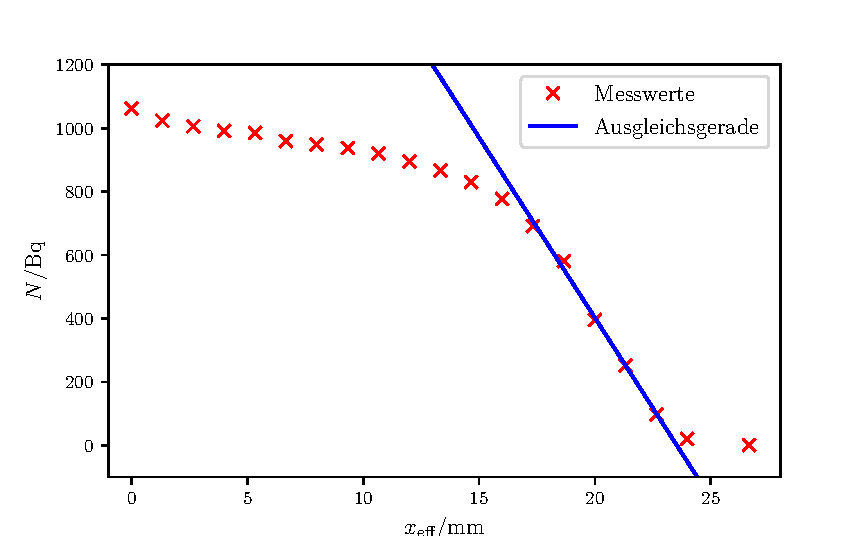
\includegraphics[width=\linewidth-70pt,height=\textheight-70pt,keepaspectratio]{content/images/Graph1N.pdf}
	\label{fig:1N}
\end{figure}
\begin{figure}
	\centering
	\caption{Die Energie $E_1$ aufgetragen gegen die effektive Länge $x_.{eff1}$.}
	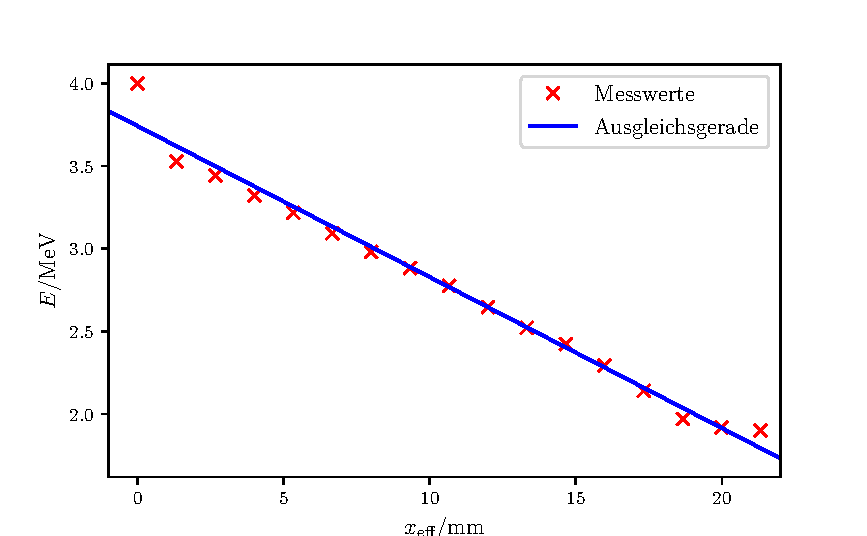
\includegraphics[width=\linewidth-70pt,height=\textheight-70pt,keepaspectratio]{content/images/Graph1E.pdf}
	\label{fig:1E}
\end{figure}

\subsection{Bestimmung der Reichweite von Alpha-Strahlung Messung 2}

Bei der zweiten Messung ist die Probe $\SI{1}{\centi\metre}$ vom Detektor entfernt.
In Abbildung \ref{fig:2N} ist mit den Werten aus Tabelle \ref{tab:2} die Impulsrate $N_2$ der zweiten Messung gegen die effektive Laufzeit $x_.{eff2}$ aufgetragen, welche nach Formel \eqref{eq:x} bestimmt wird. Eine Ausgleichsrechnung zur Bestimmung von $R_m$ und $E_\alpha$ wie in der ersten Messreihe kann aufgrund der Messdaten nicht durchgeführt werden.\\
In Abbildung \ref{fig:2E} ist mit den Werten aus Tabelle \ref{tab:2} die Energie $E_2$ der zweiten Messung gegen die effektive Laufzeit $x_.{eff2}$ aufgetragen.
Mittels einer linearen Ausgleichsrechnung der Form $E(x_.{eff})=m_2 x_.{eff} +n_2$ ergibt sich für den Energieverlust $\frac{.dE_2}{.dx}$:
\begin{align*}
\frac{.dE_2}{.dx}	&= m_2 = \SI{-118(1)}{\mega e\volt\per\metre}\text{,}\\
n_2	&= \SI{3.98(1)e6}{\becquerel}\text{.}
\end{align*}

\begin{table}
	\centering
	\caption{Der Druck $p$ und die Impulsrate $N_2$, sowie die effektiven Längen $x_.{eff2}$ und die bestimmten Energien $E_2$ bei der zweiten Messreihe mit einem Abstand zur Probe von $\SI{1}{\centi\metre}$.}
	\label{tab:tab2}
	\sisetup{table-format=1.2}
	\begin{tabular}{S[table-format=1.2]S[table-format=2.0]}
		\toprule
		{$\Delta p/\si{\bar}$} & {$N$} \\
		\midrule
		0.80 & 39 \\
		0.80 & 30 \\
		0.80 & 33 \\
		0.80 & 33 \\
		0.80 & 33 \\
		0.80 & 34 \\
		0.80 & 33 \\
		0.80 & 33 \\
		\bottomrule
	\end{tabular}

	\label{tab:2}
\end{table}
\begin{figure}
	\centering
	\caption{Die Impulsrate $N_2$ aufgetragen gegen die effektive Länge $x_.{eff2}$.}
	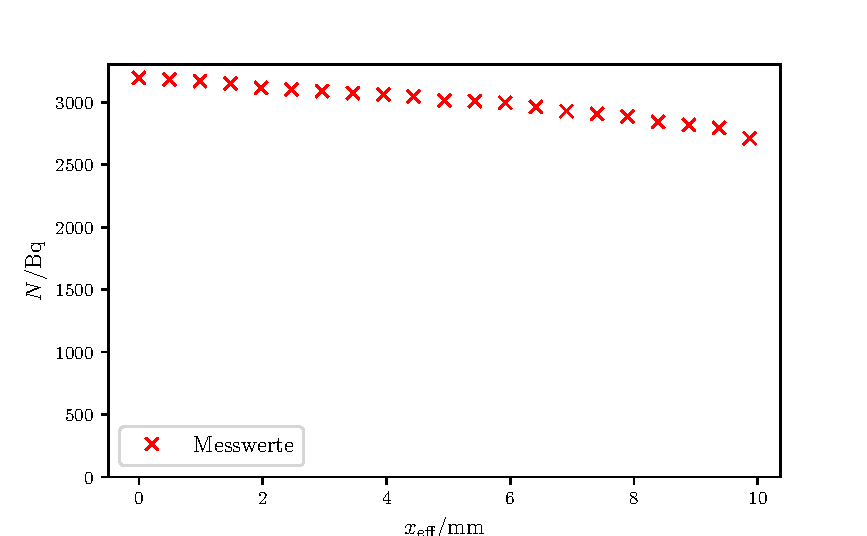
\includegraphics[width=\linewidth-70pt,height=\textheight-70pt,keepaspectratio]{content/images/Graph2N.pdf}
	\label{fig:2N}
\end{figure}
\begin{figure}
	\centering
	\caption{Die Energie $E_2$ aufgetragen gegen die effektive Länge $x_.{eff2}$.}
	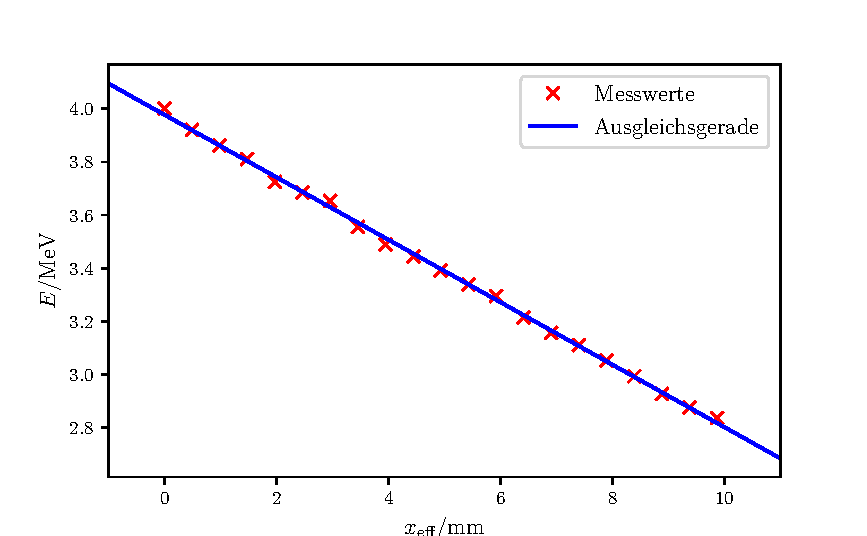
\includegraphics[width=\linewidth-70pt,height=\textheight-70pt,keepaspectratio]{content/images/Graph2E.pdf}
	\label{fig:2E}
\end{figure}

\subsection{Statistik des Radioaktiven Zerfalls}

Aus den gemessenen Zählraten ergibt sich mit der Formel für den Mittelwert
\begin{equation*}
\mu_N= \frac{1}{n}\sum_{k=1}^n N_k = \SI{671}{\becquerel}
\end{equation*} 
und die Standartabweichung
\begin{equation*}
\sigma_N=\sqrt{\frac{1}{n^2-n}\sum_{k=1}^n (N_k-\bar{N})^2)} = \SI{19}{\becquerel}
\end{equation*} 
für die mittlere Zählrate ein Wert von:
\begin{equation*}
\bar{N}= \SI{671(19)}{\becquerel} \text{.}
\end{equation*} 
Mit diesen Werten ergibt sich die Gaußverteilung gemäß:
\begin{equation*}
G(x) = \frac{1}{\sqrt{2\pi\sigma_N^2}}\exp{\left(-\frac{(x-\mu_N)^2}{2\sigma_N^2}\right)}
\end{equation*} 
und die Poissonverteilung gemäß:
\begin{equation*}
P(x) = \frac{\mu_N^x}{x!}\exp{\left(-\mu_N\right)}\text{.}
\end{equation*} 
Die Häufigkeit eines Pulses ist in den Abbildungen \ref{fig:3_20} bis \ref{fig:3_scott} für verschiedene $\Delta N$ gegen die Impulsrate $N$ aufgetragen. 

\begin{figure}
	\centering
	\caption{Die normierte Häufigkeit aufgetragen gegen die Impulsrate $N$, sowie die zugehörige Poisson- und Gaußverteilung bei einem $\Delta N$ von 20.}
	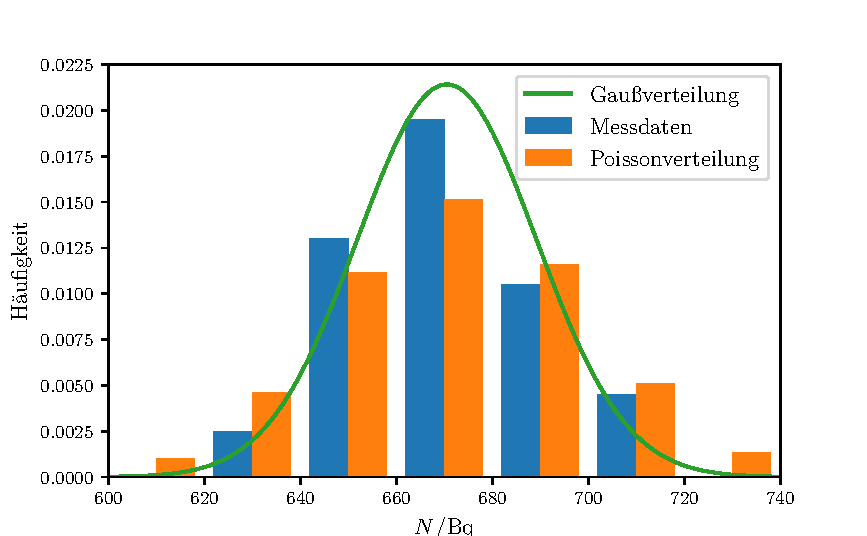
\includegraphics[width=\linewidth-70pt,height=\textheight-70pt,keepaspectratio]{content/images/Graph3_20.pdf}
	\label{fig:3_20}
\end{figure}
\begin{figure}
	\centering
	\caption{Die normierte Häufigkeit aufgetragen gegen die Impulsrate $N$, sowie die zugehörige Poisson- und Gaußverteilung bei einem $\Delta N$ von 10.}
	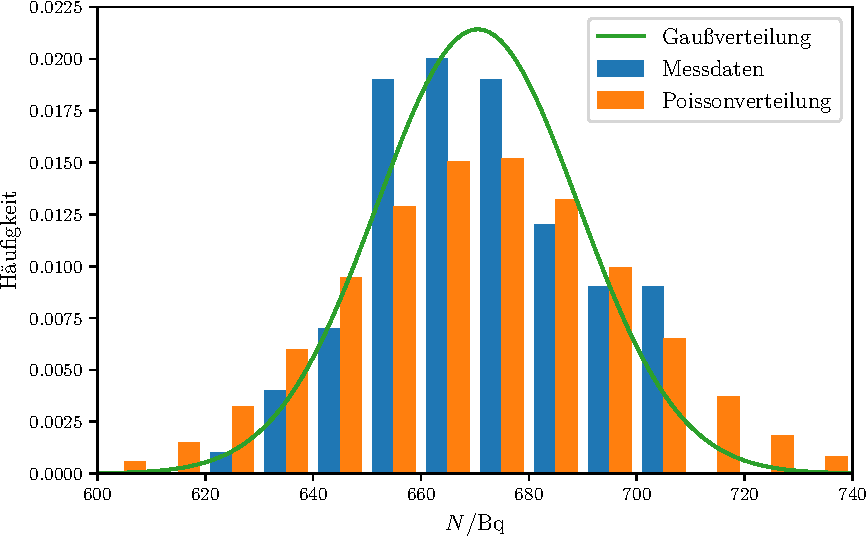
\includegraphics[width=\linewidth-70pt,height=\textheight-70pt,keepaspectratio]{content/images/Graph3_10.pdf}
	\label{fig:3_10}
\end{figure}
\begin{figure}
	\centering
	\caption{Die normierte Häufigkeit aufgetragen gegen die Impulsrate $N$, sowie die zugehörige Poisson- und Gaußverteilung bei einem weiteren $\Delta N$.}
	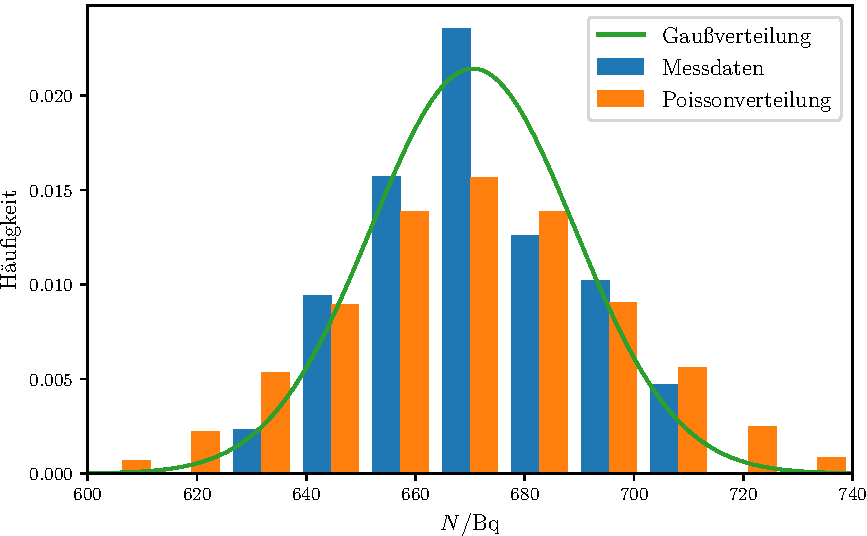
\includegraphics[width=\linewidth-70pt,height=\textheight-70pt,keepaspectratio]{content/images/Graph3_scott.pdf}
	\label{fig:3_scott}
\end{figure}
